\documentclass{article}
\usepackage[UTF8]{ctex}
\usepackage{geometry}
\usepackage{natbib}
\geometry{left=3.18cm,right=3.18cm,top=2.54cm,bottom=2.54cm}
\usepackage{graphicx}
\pagestyle{plain}	
\usepackage{setspace}
\usepackage{caption2}
\usepackage{datetime} %日期
\renewcommand{\today}{\number\year 年 \number\month 月 \number\day 日}
\renewcommand{\captionlabelfont}{\small}
\renewcommand{\captionfont}{\small}
\begin{document}

\begin{figure}
    \centering
    
\includegraphics[width=8cm]{upc.png}

    \label{figupc}
\end{figure}

	\begin{center}
		\quad \\
		\quad \\
		\heiti \fontsize{45}{17} \quad \quad \quad 
		\vskip 1.5cm
		\heiti \zihao{2} 《计算科学导论》课程总结报告
	\end{center}
	\vskip 2.0cm
		
	\begin{quotation}
% 	\begin{center}
		\doublespacing
		
        \zihao{4}\par\setlength\parindent{7em}
		\quad 

		学生姓名:\underline{\qquad  周时 \qquad \qquad}

		学\hspace{0.61cm} 号:\underline{\qquad 1907010118\qquad}
		
		专业班级:\underline{\qquad 计科1901 \qquad  }
		
        学\hspace{0.61cm} 院:\underline{计算机科学与技术学院}
% 	\end{center}
		\vskip 2cm
		\centering
		\begin{table}[h]
            \centering 
            \zihao{4}
            \begin{tabular}{|c|c|c|c|c|c|c|}
            % 这里的rl 与表格对应可以看到,姓名是r,右对齐的;学号是l,左对齐的;若想居中,使用c关键字。
                \hline
                课程认识 & 问题思 考 & 格式规范  & IT工具  & Latex附加  & 总分 & 评阅教师 \\
                30\% & 30\% & 20\% & 20\% & 10\% &  &  \\
                \hline
                 & & & & & &\\
                & & & & & &\\
                \hline
            \end{tabular}
        \end{table}
		\vskip 2cm
		\today
	\end{quotation}

\thispagestyle{empty}
\newpage
\setcounter{page}{1}
% 在这之前是封面,在这之后是正文
\section{引言}
	从小,我对计算机的兴趣,或是说对所有新科技新事物都有极其浓烈的的兴趣,但是因为身边的人没有任何从事技术相关行业的,所以我对计算机从来都是一知半解,虽然身边的亲戚朋友或者老师同学出现技术上的问题总是会叫我去解决,但是我知道,我对计算机技术只不过是了解了一点皮毛,没有深入的去理解,是计算机科学与技术导论带我深入的了解整个计算机理论的发展历程和大概的组成框架,让我了解到作为一个计算机技术相关的学生以及即将走向工作岗位的中国技术人我应当承担哪些为国奉献的责任。\par
	通过对比特币的调研,我更是认识到了一名技术人投机取巧是非常不可取的,我们要像华为的总裁任正非那样,从基础抓起,从根源入手,居安思危,即使是在经济高度全球化的今天,我们也不能放松对于核心技术掌控的意识,更是要有大局观,不能只看眼前的一隅之地,要从时间和空间纵深准备,这样才能够让一个人、一个公司乃至一个国家更加长久的存在下去。\par


\section{对计算科学导论这门课程的认识、体会}
\begin{itemize}
    
    \item 计算机导论课让我们学习如下内容:

一、计算科学的基础概念和基本知识

二、计算机科学:它的意义、内容和方法

三、如何学习计算科学和健康成长

四、布尔代数基础

除此之外,我们还学习了大量的技术名词及其背后的含义,通过长达数个星期的PPT讲解与调研,我对各个技术都有了大概的了解,这是我对未来的方向更加的明确,对行情更加的了解,而不是作为一个只安于自己一隅的技术研究者,我认识到要成为一名出色的计算机工作者,单单是了解一门技术是不够的,必须要加强自己在公司中的不可替代性,这样我们才不会遇到IT行业惯有的“中年危机”。\par

    \item 对《计算机导论》这门课程,我的感觉是:\par
	计算机科学与技术导论不仅仅是对计算机技术发展历程与组成的简单概括,他更是对新一代技术人的启蒙宝典,也是领路人。学完了计算机科学与技术导论,我认识到了我以前对计算机的人是有多么肤浅,更是让我对自己未来的规划有了更加清晰明了的认识。\par

\end{itemize}
\par

\section{进一步的思考}

	这次,我和我的搭档所调研的题目是比特币,提到比特币我们都或多或少有所耳闻,比特币这个词语被涂抹上上了很多神秘色彩,一夜暴富,新科技,新的货币,一个又一个的标签使比特币自从诞生以来一直备受关注。\par
	\subsection{创始人背后的故事}
	 在此次调研中,我和我的搭档深入的调研了比特币对社会与经济的意义,以及他的根本性质(即比特币究竟是属于货币还是属于财产),但是对比特币的创始人中本聪却没有太放在心上,所以在此会详细叙述一下我对于比特币创始人中本聪的调查。\par
	中本聪的地位比密码学货币的先行者大卫·乔姆还要要高,而但是其他的同行科技人员由于原来经历过的数字货币失败,多半人对比特币抱有悲观态度。\par
	中本聪不像凯文那样对密码学货币领域那些失败的前辈顶礼膜拜,相反,他对“现在更多的人对90年代感兴趣”不以为然,在与一位研究者的信件交流中,他强调比特币的独一无二,嘲弄基于“信任第三方”系统的失败(例如电子现金)。“我希望人们能够有一种区别,即人们认为“我是第一次知道我们在尝试一个无信任第三方为基础的系统”。”中本聪的自信可见一斑。\par
	中本聪对这些失败者的反省是,Beenz、Flooz、E-cash、B-money等虚拟货币先驱尝试的失败主要是由其中心化的组织结构所造成的。这是因为一旦为虚拟货币信用背书的公司倒闭,或保管总账的中央服务器被黑客攻破,该虚拟货币即面临信用破产与内部崩溃的风险。2009年2月,中本聪在IRC频道写道:“政府擅长击溃Napster那样拥有中央控制的网络,但是Gnutella 和Tor 这样完全P2P的网络看起来依旧安枕无忧。” (《比特币:一个虚幻而真实的金融世界》预计在2013年12月15日上市,巴比特成员合著,京东、当当已有预售)\par
	中本聪的密码学造诣十分精湛,许多曾经被认为是冗余设计的错误,后来被证明都是正确的,比如精心挑选的Koblitz曲线,避开了美国国安局在加密标准中暗藏的后门。比如在椭圆曲线数字签名算法加密的基础上,再哈希两次,足以应付量子计算机的威胁……(中本聪的天才:比特币以意想不到的方式躲开了一些密码学子弹)\par
	中本聪为上线比特币项目,精心准备了身份资料与域名。早在2008年8月18号就注册了http-://bitcoin.org的域名,并保护性注册了http://bitcoin.net 。whois的信息都毫无价值地指向位于芬兰赫尔辛基的一家小型主机托管商。域名注册商为一家小公司http://anonymousspeech.com,为什么选择这家公司,因为这家公司的服务声称他能为用户的域名注册提供匿名性保证,确保不受人肉搜索,也不会遭到政府的检索。研究人员曾一度追踪到这家公司,结果是竹篮打水一场空。因为中本聪使用Tor网络发送邮件,而且,目前 http://bitcoin.org 大概已经移交了所有权,这也是为什么移到了赫尔辛基的原因。但是 http://bitcoin.net 这个域名一定还在Satoshi的手里。完成域名准备工作之后,中本聪这才于2009年2月11日,在http://p2pfoundation.ning.com发起“比特币”这一项目。\par
	意味深长的是,中本聪在创世区块里留下一句永不可修改的话:“The Times 03/Jan/2009 Chancellor on brink of second bailout for banks,当时正是英国的财政大臣达林被迫考虑第二次出手纾解银行危机的时刻。”这句话是泰晤士报当天的头版文章标题。中本聪引用这句话,既是对该区块产生时间的说明,又是对金融危机中旧有的脆弱银行系统的冷嘲,还可能是一个对其身份的猜测鄙视。人们可能误解了比特币诞生的意义,在白皮书《比特币:一种点对点的电子现金系统》中,中本聪甚至提都没提“货币”这个词,而存在性证明,却在创世区块就已经暗示了。直到几年之后,社区开发者才意识到区块链的深远意义。\par
	中本聪行事缜密细致,与任何人交流都使用PGP加密和Tor网络。加文·安德列森(比特币基金会首席科学家)曾向记者透露,有很多人都冒充中本聪写信给他,但被他轻易识破,因为他们没有使用PGP加密。中本聪哪怕与最亲密的合作伙伴交流也使用加密,而且从不透露个人信息,加文、尼克·萨博、哈尔芬尼均对他知之甚少。中本聪把项目的领导权移交给加文,仅仅是通过邮件的简短交流。联想丝绸之路站长被FBI安排的卧底钓鱼,中本聪显然要高明得多。他甚至在白皮书和社区发言中,有意的伪造一些身份信息与个性化特征,误导一些错误的猜测。比如伪装英式拼读,格林威治时间的作息规律,日本名字,论文中“WE”的第一人称,使用生僻的科技术语,模仿密码学同仁的写作风格,反复使用‘of course’无逗号隔离,不同于惯用的方法(‘the problem of course is’);使用‘preclude’一词(仅在1.5\%的密码论文中出现)……他的这些障眼法取得了不错的效果,已经有无数研究者、情报人员调查过他的真实身份,候选人多达几十位,有天才数学家,有技术大牛,还可能是团队,但没有一个得到核实。(分析称比特币之父中本聪或为经济学教授尼克萨博,业内人士质疑中本聪或为京都大学教授望月新一)\par
	前段时间两位以色列计算机专家曝料,发现比特币黑市网站“丝绸之路”站长罗斯威廉乌布利希与中本聪可能存在财务往来,这不禁让人为中本聪捏一把汗,所幸的是,中本聪没有犯这么愚蠢的错误。很快有人站出来,澄清那个地址是他的,不是中本聪的。中本聪从未动用早期挖矿所得的比特币,这些币就像是雅浦岛渔民不小心遗落大海里的石币一样,永久地沉默着。对此,FBI无可奈何。他们的心情就跟高效密码学组标准现任主席Dan Brown得知比特币使用secp256k1时一样,意外中夹杂着沮丧。中情局雇员斯诺登不久前披露NSA(国安局)在椭圆曲线算法(ECC)中埋了个陷阱,他们知道不为人知的方法来弱化这条曲线。但是很遗憾,比特币让他们失望了,中本聪使用的不是NSA精心挑选的伪随机曲线,而是Koblitz曲线。中本聪怎么知道国际通用加密标准ECC中有后门,恐怕只有天知道了。\par
	作为顶级黑客,不能在互联网隐藏自己的身份,这本身已构成一个怀疑。\par
\subsection{对比特币的进一步思考之央行虚拟货币}
\begin{itemize}
\item 虚拟货币监管\par
比特币号称「币」,所以各国货币当局都在严肃思考:它是不是一种货币,怎么应对,怎么监管。目前逐渐形成的共识是,比特币的资产属性大于货币属性,依据来源于它的两个特性。\par

一是更多被用于炒作,而非支付。很少人真正用比特币去支付。因为比特币支付耗费的时间很长,若用比特币买杯咖啡,买的时候是热的,喝的时候可能就凉了。二是价格波动太大,每天都是上下几百美元的波动。货币本来就是一把尺子,是一个计算单位,若这个尺子每天变长变短,就无法正确度量商品的价格。目前比特币是一个不固定的测量单位,所以许多人认为它无法成为真正的货币。\par

比特币更多是一种数字资产。从某种意义上来说,有一时间段数字资产比其他资产的投资回报都要高,这也是为什么全球许多投资公司非常重视这一领域。目前,像比特币这样的虚拟货币,全球有几千种,而数字资产交易所却开了一万多家,可见这个领域的交易多么火爆,许多人觉得这个生意可以赚钱,因此冲进这个市场,也正因为此,各国监管当局怎么管理它,就成为一个很重要的问题。\par

怎么管,首先涉及怎么定性,如果把它定义成货币,那就依照货币的管理办法。如果说它是一个资产,那就依照资产的管理办法。如果说它是一个商品,那就依照商品的管理办法。定性不同,决定了管理办法和部门的不同。\par

应该说,虚拟货币是一个全新的事物,各国的监管态度和争议颇大。目前看,将它归类为证券的可能性较大,但这也有一个过程,尚未有最后定论。在美国,目前监管虚拟货币的部门有两个:一个是美国证监会;另一个是美国商品期货交易委员会,它把虚拟货币当作商品来看。到底是谁来管,美国监管部门正在加快确定。在金融这个领域,各国还是主要跟随美国的。一旦美国把虚拟货币定性了,全球就会向美国看齐。\par

目前,我国把虚拟货币当成邮票一样的物品来管理,且严禁以代币为融资标的进行融资活动,尤其是初始代币发行(Initial Coin Offerings,ICO)。数据显示,全球 ICO 融资总额正逐年上涨,主要发生地在美国。相比较,美国的 ICO 项目还是靠谱居多,而国内的 ICO 项目基本以骗子为主,99\% 项目不靠谱。就某种程度而言,我们的政策似乎有点一刀切,但有它的苦衷和合理之处。在我国,有一些不法分子钻空子、造假、金融欺诈、非法融资,严重损害投资者利益和金融秩序,因此应严加惩治。\par
\item 央行数字货币\par
40 年来加密货币的不断发展,带来了当前全球性的大规模数字加密货币试验,这也使各个中央银行不得不严肃考虑一个问题:中央银行是不是也应该发行数字货币。\par

我国是最早研究央行数字货币的国家之一,在 2014 年就开始着手。研究央行数字货币首先须回答一个有意思的问题,什么叫央行数字货币。对此,各国目前还没有形成一个统一的共识,2018 年,国际清算银行(Bank for International Settlements,BIS)的一篇报告给出了一个比较有意思的定义,不过它不是正面回答这个问题,而使用了一种排除法来进行定义。它将目前存在的各类支付工具进行了汇总,然后判定哪些不是央行数字货币,一一排除后,剩下的就是央行数字货币。\par

它使用了四个维度的标准:是不是可以广泛获得、是不是数字形式、是不是中央银行发行的、是不是类似比特币这种技术产生的代币。按照这四个维度,现金是可以广泛获得的,非数字化的,中央银行发行的,以代币形式存在的货币。银行存款是可以广泛获得的,数字化的,非中央银行发行的,不是代币形式的货币。它们都不是央行数字货币。除了现金,中央银行发行的货币还有银行准备金,包括存款准备金、超额存款准备金。银行准备金已经数字化,但是 BIS 认为,这不是中央银行所要真正研究的央行数字货币。\par

一种可能的央行数字货币是中央银行的账户向社会公众开放,允许社会公众像商业银行一样在中央银行开户,这个好理解,相当于中央银行开发了一个超级支付宝,面向所有的 C 端客户服务。BIS 认为这样形成的央行货币是央行数字货币,将其称为基于账户(Account)的央行数字货币,或称 CBDA(Central Bank Digital Account)。另一种可能的央行数字货币是中央银行以比特币这种技术发行的代币,可称为基于代币(Token)的央行数字货币,或称 CBCC(Central bank Cryptocurrency,CBCC),这类货币既可以面向批发,也可以面向零售。基于账户还是基于代币,代表了两种不同的技术路线,哪种思路未来将占据主流,还有待观察。\par

在技术架构上,央行数字货币体系可分为两类:一元体系和二元体系。一元体系是指中央银行以类似超级支付宝的方式直接为客户提供服务,但世界大多数中央银行并不认可这一方式,不愿意直接向公众提供央行数字货币服务,而是希望复用传统金融体系,与金融机构合作,将中央银行置于后端,前端的服务则交由金融机构提供。中国人民银行提出的二元体系即是这一思路,国际上称之为双重架构,这一思路正逐渐形成各国的共识。无论是一元体系还是二元体系,都是数字货币在金融体系内展开的思路,现在比较热的稳定代币,尤其是锚定法币的数字稳定代币,则是在传统金融体系之外,以增量的方式展开的思路。\par

当前,中国人民银行正在开展央行数字货币研发试验。由于第三方支付的异军突起,我国的账户体系走在全世界前列。但实际上,有人认为,真正代表未来技术发展方向的央行数字货币应是基于加密货币技术的央行数字货币,即 CBCC,目前学界和业界均在积极开展 CBCC 模式的探索,许多人认为,CBCC 可以让客户真正自主管理自己的钱,而不是交给第三方,真正赋予了客户自主的权利。虽然尚不能肯定它一定就是将来的方向,但至少目前来看,这是最热的前沿焦点。\par
\end{itemize}
\section{总结}
这次的计算科学导论的作业完成,对于我这个今年刚刚入学的、以前几乎未接触过技术的大一学生来说,可以说是艰难曲折,无论是对于一个具体的课题的调研还是在LaTex上论文的编写,对于我来说就是一道又一道的等待我去翻越的山峰。最终我也克服了重重困难,LaTeX环境的配置足足花了我接近两天的时间,最晚的时候熬到了凌晨两点,我学到了很多。虽然看似很累,但是真的在自己技术探索的道路上迈出了坚实而有力的第一步。希望在未来的日子里,我能够不忘初心,保持对技术的热爱与渴望,做一个负责任、有理想、有担当道德新时代中国技术人!


\section{附录}
\begin{itemize}

\begin{figure}[htb!]
\item\subsection{Github}
\centering
\includegraphics[scale=0.2]{Github}
\caption{Github网址:https://github.com/libaohui179793/-}
\label{fig:Github}
\end{figure}

\begin{figure}[htb!]
\item\subsection{观察者}
\centering
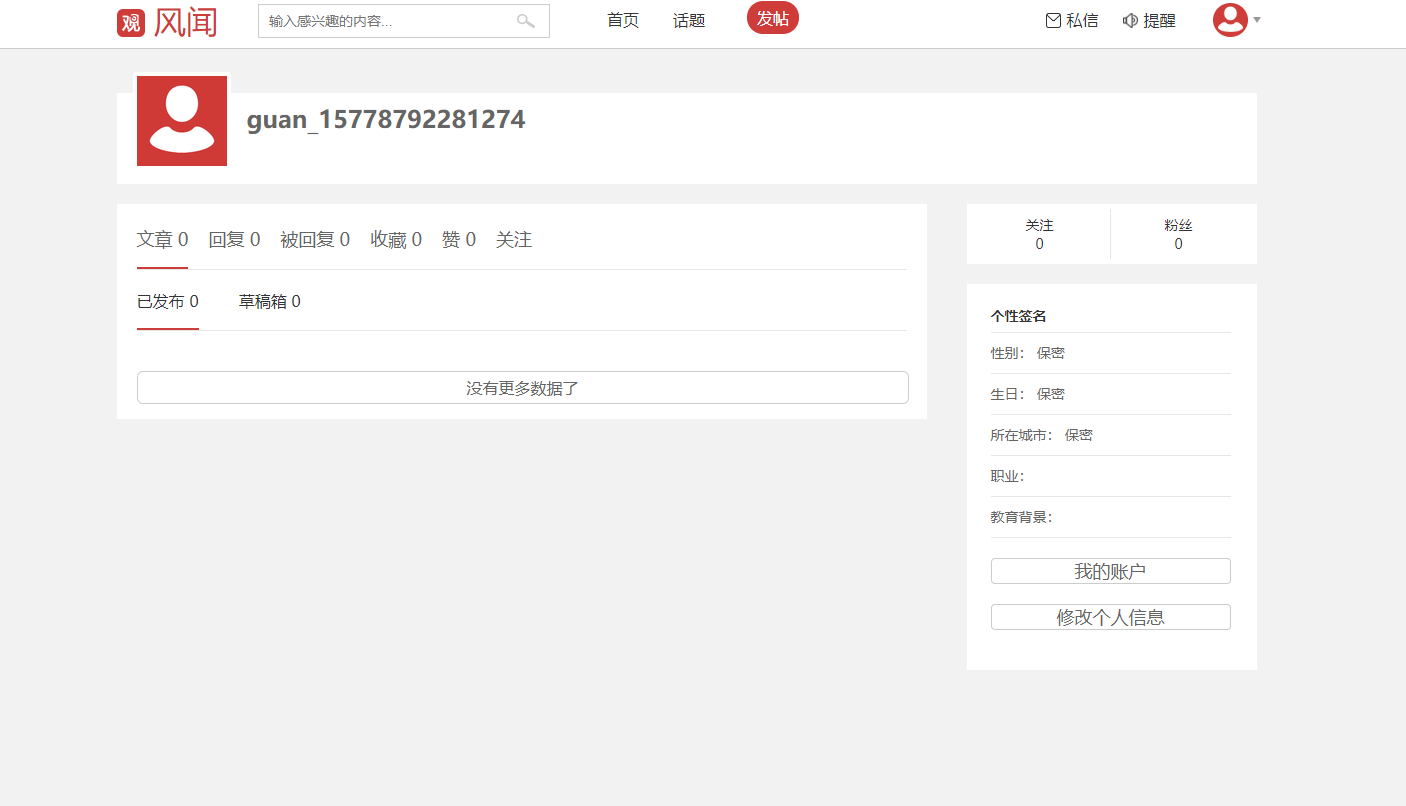
\includegraphics[scale=0.3]{guanchazhe}
\caption{观察者}
\label{fig:guanchazhe}
\end{figure}

\begin{figure}[htb!]
\item\subsection{学习强国}
\centering
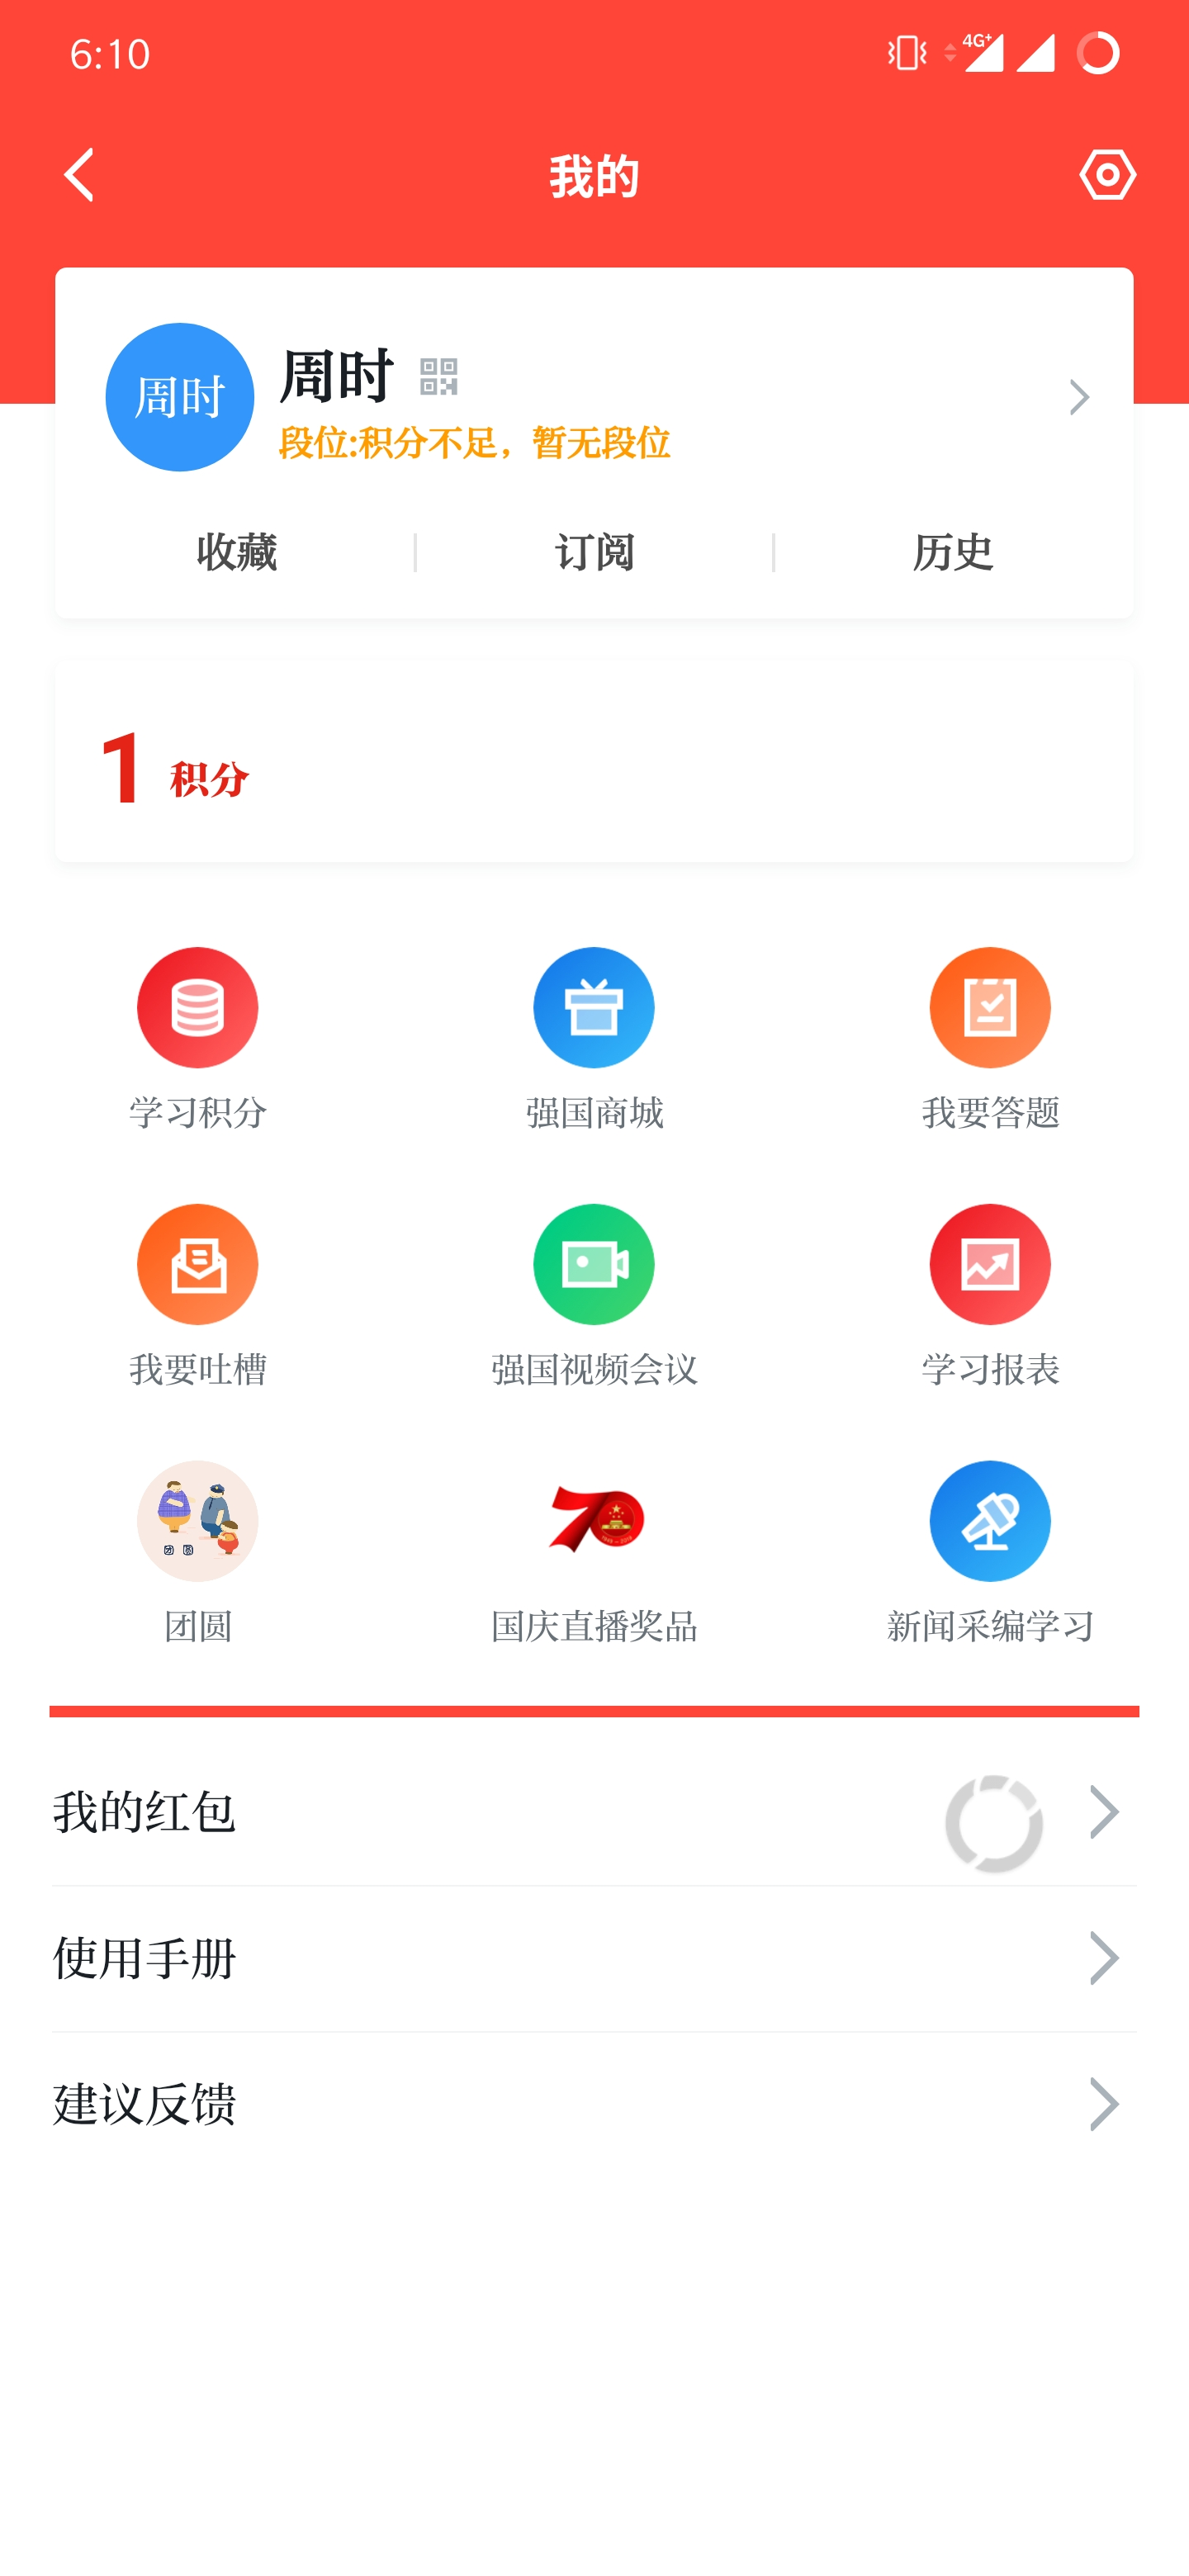
\includegraphics[scale=0.25]{xuexiqiangguo}
\caption{学习强国}
\label{fig:xuexiqiangguo}
\end{figure}

\begin{figure}[htb!]
\item\subsection{bilibili}
\centering

\includegraphics[scale=0.25]{bilibili}
\caption{bilibili}
\label{fig:bilibili}
\end{figure}

\begin{figure}[htb!]
\item\subsection{CSDN}
\centering
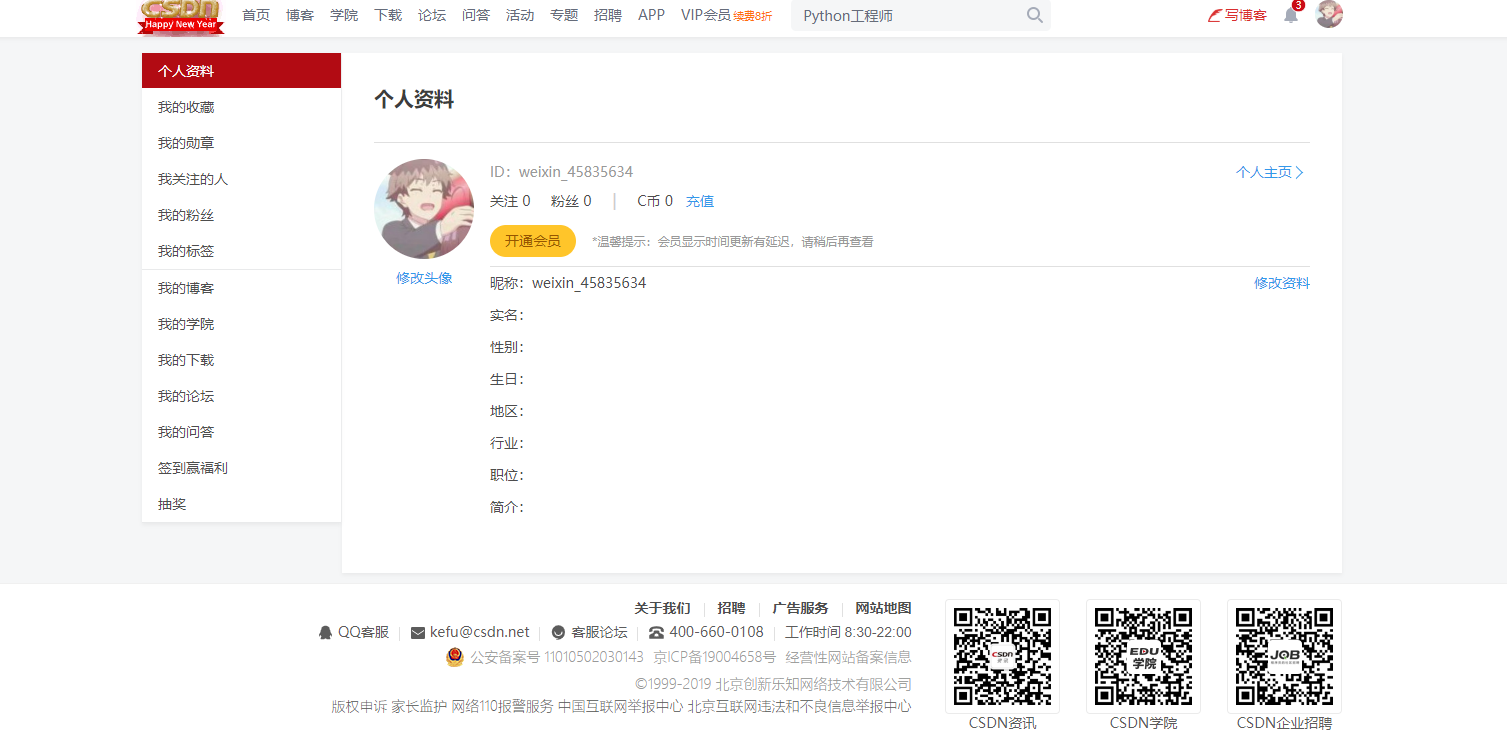
\includegraphics[scale=0.25]{CSDN}
\caption{CSDN网址:https://i.csdn.net/\#/uc/profile}
\label{fig:CSDN}
\end{figure}

\begin{figure}[htb!]
\item\subsection{博客网}
\centering
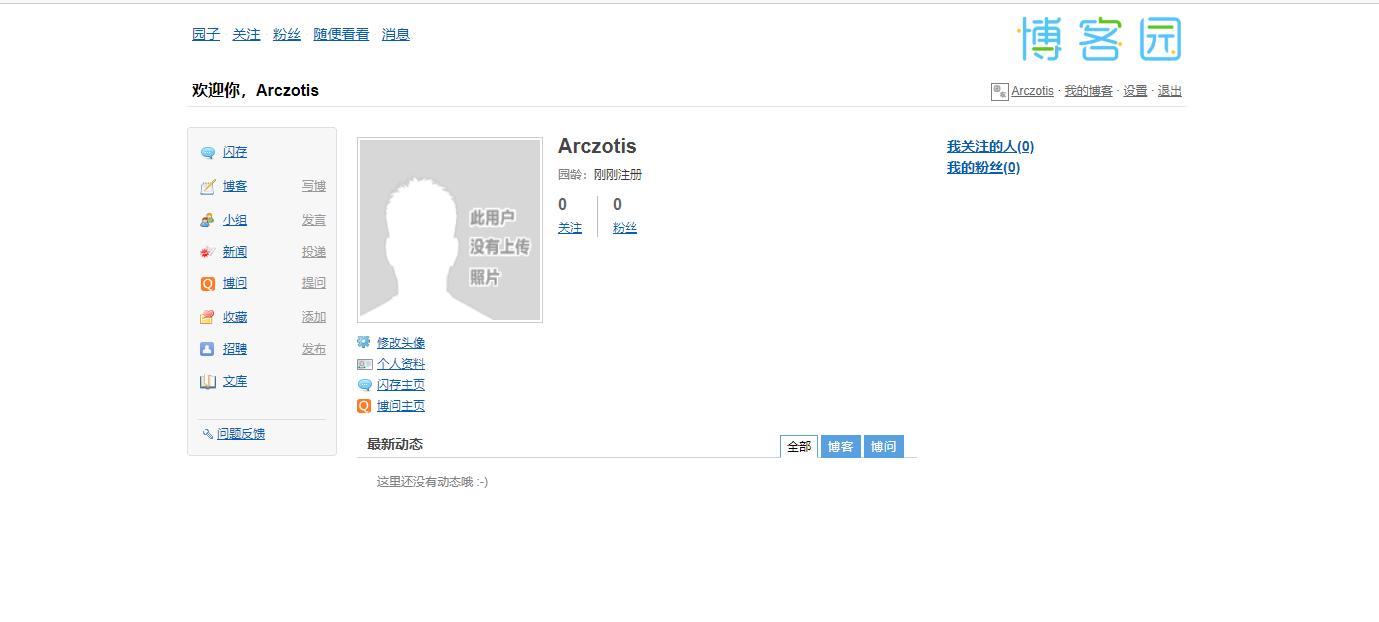
\includegraphics[scale=0.25]{bokeyuan}
\caption{博客园网址:https://home.cnblogs.com/}
\label{fig:bokeyuan}
\end{figure}

\begin{figure}[htb!]
\item\subsection{小木虫}
\centering
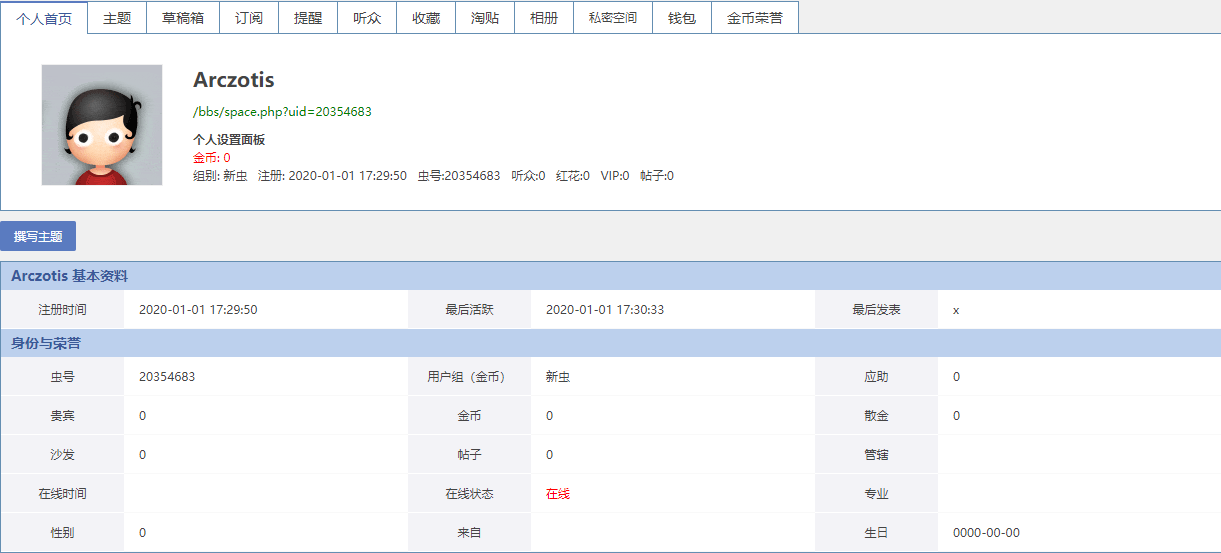
\includegraphics[scale=0.25]{xiaomuchong}
\caption{小木虫网址:http://muchong.com/bbs/space.php?uid=20254043}
\label{fig:xiaomuchong}
\end{figure}

\end{itemize}

\end{document}
